\documentclass{article}
\usepackage{../assignment_preamble}

\title{Homework 2}
\author{Ravi Kini}
\date{November 3, 2025}

\begin{document}

\maketitle

\problem{}
Let $A$ be a $m \times n$ strictly column diagonally dominant matrix. Then for all $k$:
\begin{align*}
    |A_{kk}| > \sum_{i \neq k} |A_{ik}|
\end{align*}
For Gaussian elimination with partial pivoting, row $k$ of matrix $A$ is interchanged only when for some $i > k$:
\begin{align*}
    |A_{k,k}| \geq |A_{i,k}|
\end{align*}
Note that for strictly column diagonally dominant matrices, no row interchange occurs since $|A_{kk}| > \sum_{i \neq k} |A_{ik}| > |A_{jk}|$ for all $j, k$. It then follows that after $k$ steps of Gaussian elimination, if the submatrix excluding the first $k$ columns/rows is strictly column diagonally dominant, no row interchange occurs for the $k + 1$th step. Let $A^{(k)}$ denote the matrix after the $k$th step of Gaussian elimination is performed (i.e., $A^{(0)} = A$). We show by induction that after the $k$th step, the submatrix excluding the first $k$ columns/rows is strictly column diagonally dominant; since $A$ is already strictly column diagonally dominant, the base case of $k = 0$ holds. Suppose after the $k - 1$th step, the hypothesis holds. We can then select the $k$th row as the pivot row, and $A^{(k-1)}_{k,k}$ as the pivot element. Then, for all $i > k$, using the triangle inequality:
\begin{align*}
    \sum_{j > k, j \neq i} |A^{(k)}_{j,i}| & = \sum_{j > k, j \neq i} \left|A^{(k - 1)}_{j,i} - A^{(k-1)}_{j,k}\frac{A^{(k-1)}_{k,i}}{A^{(k-1)}_{k,k}}\right| \\
    & \leq \sum_{j > k, j \neq i} |A^{(k - 1)}_{j,i}| + \sum_{j > k, j \neq i}|A^{(k-1)}_{j,k}|\frac{|A^{(k-1)}_{k,i}|}{|A^{(k-1)}_{k,k}|} \\
    & \leq \sum_{j > k, j \neq i} |A^{(k - 1)}_{j,i}| + |A^{(k-1)}_{k,i}| \frac{\sum_{j > k, j \neq i} |A^{(k-1)}_{j,k}|}{|A^{(k-1)}_{k,k}|} \\
    & \leq \sum_{j \geq k, j \neq i} |A^{(k - 1)}_{j,i}| - |A^{(k - 1)}_{j,k}| + |A^{(k-1)}_{k,i}| \frac{\sum_{j > k} |A^{(k-1)}_{j,k}| - |A^{(k-1)}_{i,k}|}{|A^{(k-1)}_{k,k}|} \\
\end{align*}
Using the strict column diagonal dominance of the submatrix of $A^{(k-1)}$ that excludes the first $k - 1$ columns/rows:
\begin{align*}
    \sum_{j > k, j \neq i} |A^{(k)}_{j,i}| & \leq |A^{(k - 1)}_{i,i}| - |A^{(k - 1)}_{k,i}| + |A^{(k-1)}_{k,i}| \frac{|A^{(k-1)}_{k,k}| - |A^{(k-1)}_{i,k}|}{|A^{(k-1)}_{k,k}|} \\
    & \leq |A^{(k - 1)}_{i,i}| - |A^{(k - 1)}_{k,i}| + |A^{(k-1)}_{k,i}|\left(1 - \frac{|A^{(k-1)}_{i,k}|}{|A^{(k-1)}_{k,k}|}\right) \\
    & \leq |A^{(k - 1)}_{i,i}| - |A^{(k-1)}_{k,i}\frac{|A^{(k-1)}_{i,k}|}{|A^{(k-1)}_{k,k}|} \\
    & \leq \left|A^{(k - 1)}_{i,i} - A^{(k-1)}_{k,i}\frac{A^{(k-1)}_{i,k}}{A^{(k-1)}_{k,k}}\right| \\
    & \leq |A^{(k)}_{i,i}|
\end{align*}
The submatrix of $A^{(k)}$ that excludes the first $k$ columns/rows is then strictly column diagonally dominant. By induction, this holds for every step of Gaussian elimination, and so row interchange does not occur when performing Gaussian elimination on a strictly column diagonally dominant matrix.

\clearpage
\problem{}
\subproblem{(a)}
\begin{lstlisting}[language=Python]
import numpy as np
import matplotlib.pyplot as plt
import random

N = 10 ** 3

min_exp, max_exp = 1, 6

rel_error_arr = np.empty((max_exp - min_exp + 1, N))
kappa_arr = np.empty((max_exp - min_exp + 1, N))

for j in range(max_exp - min_exp + 1):
    for i in range(N):
        n = 2 ** j
        A = np.random.rand(n, n) * 2 - 1
        z = np.random.rand(n, 1) * 2 - 1
        b = np.matmul(A, z)
        x = np.linalg.solve(A, b)
        kappa = np.linalg.cond(A)
        rel_error = np.linalg.norm(x - z) / np.linalg.norm(z)
        rel_error_arr[j][i] = rel_error
        kappa_arr[j][i] = kappa

for j in range(max_exp - min_exp + 1):
    plt.scatter(kappa_arr[j], rel_error_arr[j], label=f'n = {2 ** (min_exp + j)}')
plt.xscale('log')
plt.yscale('log')
plt.xlabel('Condition number')
plt.ylabel('Relative error')
plt.title('Relative error vs. Condition number')
plt.grid(True, which='both', ls='-')
plt.legend()
plt.show()

def fit_function(x, a, k):
  return a * x ** k
for j in range(max_exp - min_exp + 1):
  popt, pcov = sp.optimize.curve_fit(fit_function, kappa_arr[j], rel_error_arr[j])
  print(popt)
\end{lstlisting}
\begin{center}
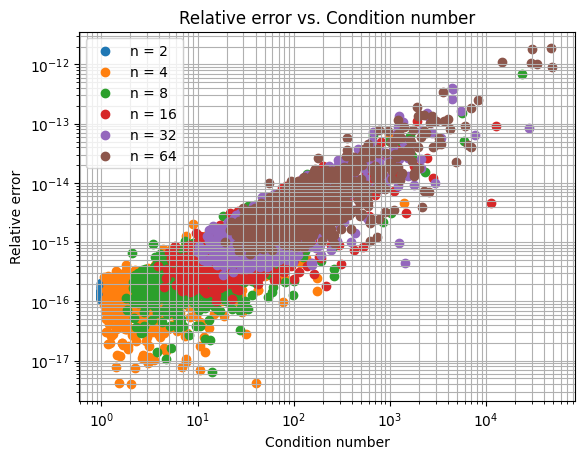
\includegraphics[width=0.6\textwidth]{../../img/mat226a_kappa_relerror_scaling.png}
\end{center}
There is a linear relationship between the logs of the condition number and of the relative error with a slope of approximately $1$, which indicates that $\frac{||x - z||}{||z||} \propto \kappa(A)$.
\subproblem{(b)}
The scaling is not dependent on the matrix size.
\subproblem{(c)}
The intercept on the log-log plot is approximately machine epsilon, which means that the constant of proportionality between the condition number and the relative error is approximately maxhine epsilon, as expected.

\clearpage
\problem{}
\begin{align*}
    \rho = \frac{\max_{i,j}|U_{i,j}|}{\max_{i,j}|A_{i,j}}
\end{align*}
\subproblem{(a)}
For a $n \times n$ matrix $A$, let $A^{(k)}$ denote the matrix after the $k$th step of Gaussian elimination is performed (i.e., $A^{(0)} = A$). We first show that $\max_{i,j}|A^{(k)}_{i,j}| \leq 2^k \max_{i,j}|A_{i,j}|$. The base case holds trivially since $\max_{i,j}|A^{(0)}_{i,j}| = \max_{i,j}|A_{i,j}|$. Suppose the bound holds for the first $k - 1$ steps. At step $k$, we choose the pivot $A^{(k-1)}_{k,k}$ such that:
\begin{align*}
    |A^{(k-1)}_{k,k}| \geq |A^{(k-1)}_{i,k}| 
\end{align*}
for all $i > k$. Consequently:
\begin{align*}
    \frac{|A^{(k-1)}_{i,k}|}{|A^{(k-1)}_{k,k}|} \leq 1
\end{align*}
For all $i \neq k$ and all $j$:
\begin{align*}
    |A^{(k)}_{i,j}| & = \left|A^{(k-1)}_{i,j} - \frac{A^{(k-1)}_{i,k}}{A^{(k-1)}_{k,k}}A^{(k-1)}_{k,j}\right| \\
    & \leq |A^{(k-1)}_{i,j}| + \left|\frac{A^{(k-1)}_{i,k}}{A^{(k-1)}_{k,k}}A^{(k-1)}_{k,j}\right| \\
    & \leq |A^{(k-1)}_{i,j}| + |A^{(k-1)}_{k,j}| \\
    & \leq 2\max_{p,q} |A^{(k-1)}_{p,q}| \\
    & \leq 2 \cdot 2^{k-1}\max_{p,q}|A_{i,j}| \\
    & \leq 2^k\max_{i,j}|A_{i,j}|
\end{align*}
For all $j$:
\begin{align*}
    |A^{(k)}_{k,j}| = |A^{(k-1)}_{k,j}| & \leq 2^{k-1}\max_{i,j}|A_{i,j}| \\
    & \leq 2^k\max_{i,j}|A_{i,j}|
\end{align*}
Therefore $\max_{i,j}|A^{(k)}_{i,j}| \leq 2^k \max_{i,j}|A_{i,j}|$, and by induction, this holds for all $k$. Note that in the LU decomposition of $A$, if $A = LU$, $U = A^{(n - 1)}$. Then:
\begin{align*}
    \max_{i,j}|U_{i,j}| = \max_{i,j}|A^{(n-1)}_{i,j}| & \leq 2^{n-1}\max_{i,j}|A_{i,j}| \\
    \rho = \frac{\max_{i,j}|U_{i,j}|}{\max_{i,j}|A_{i,j}|} & \leq 2^{n-1}
\end{align*}
\subproblem{(b)}
\begin{lstlisting}[language=Python]
import numpy as np
import matplotlib.pyplot as plt
import random
import scipy as sp

N = 10
min_exp, max_exp = 1, 12

n_arr = np.empty((max_exp - min_exp + 1) * N)
rho_arr = np.empty((max_exp - min_exp + 1) * N)

for j in range(min_exp, max_exp + 1):
  for i in range(N):
    n = 2 ** j
    A = np.random.rand(n, n) * 2 - 1
    P, L, U = sp.linalg.lu(A)
    rho = np.max(U) / np.max(A)
    n_arr[(j - 1) * N + i] = n
    rho_arr[(j - 1) * N + i] = rho

plt.scatter(n_arr, rho_arr)
plt.xscale('log')
plt.yscale('log')
plt.xlabel('Size')
plt.ylabel('Growth factor')
plt.title('Growth factor vs. Size')
plt.grid(True, which='both', ls='-')
plt.show()

def fit_function(x, a, k):
  return a * x ** k
popt, pcov = sp.optimize.curve_fit(fit_function, n_arr, rho_arr)
print(popt)
\end{lstlisting}
\begin{center}
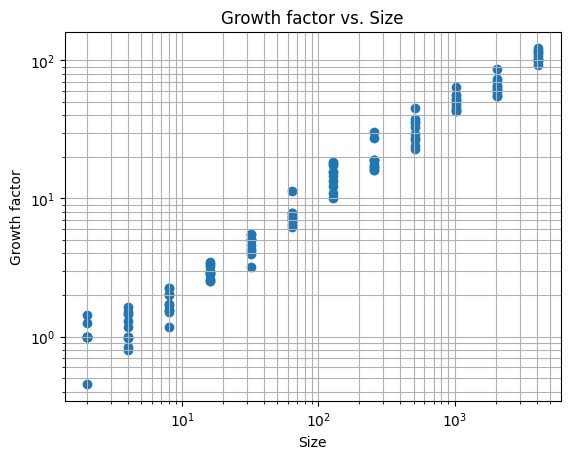
\includegraphics[width=0.6\textwidth]{../../img/mat226a_size_rho_scaling.png}
\end{center}
There is a linear relationship between the logs of the size and of the growth factor with a slope of approximately $0.6$ and intercept of approximately $0.75$, which indicates that the $\rho \approx 0.75n^{0.6}$.
\subproblem{(c)}
For a matrix of size $10^6 \times 10^6$, I expect a growth factor of about $0.75{(10^6)}^{0.6} \approx 2985.8$. This is far lower than the bound from part (a), which indicates that for most matrices, Gaussian elimination with partial pivoting is numerically stable.

\clearpage
\problem{}
\subproblem{(a)}
Let $A$ be a $m \times n$ matrix.
Let $i^*$ such that $||A||_\infty = \sum_{j=1}^n |A_{i^*,j}|$. Define the vector $x$ such that:
\begin{align*}
    x_j = \frac{\mathrm{sgn}(A_{i^*,j})}{\sqrt{n}}
\end{align*}
Evidently, $||x||_2 = n \cdot {\left(\frac{1}{\sqrt{n}}\right)}^2 = 1$. Then:
\begin{align*}
    {(Ax)}_i & = \frac{1}{\sqrt{n}}\sum_{j=1}^n |A_{i,j}| \\
    {(Ax)}_{i^*} & = \frac{||A||_\infty}{\sqrt{n}}
\end{align*}
We see that ${(Ax)}_{i^*} \geq {(Ax)}_{i}$ for all $i$. Then:
\begin{align*}
    ||A||_2 \geq ||Ax||_2 \geq {(Ax)}_{i^*} \geq \frac{||A||_\infty}{\sqrt{n}}
\end{align*}

For an arbitrary $x$ such that $||x||_2 = 1$:
\begin{align*}
    ||Ax||_2^2 = \sum_{i=1}^m \left|\sum_{j=1}^n A_{i,j}x_j\right|^2 \\
\end{align*}
By the Cauchy-Schwarz inequality:
\begin{align*}
    \left|\sum_{j=1}^n A_{i,j}x_j\right| & \leq \sum_{j=1}^n |A_{i,j}||x_j| \\
    & \leq \sum_{j=1}^n |A_{i,j}| \\
    & \leq ||A||_\infty
\end{align*}
Then:
\begin{align*}
    ||Ax||_2^2 & \leq \sum_{i=1}^m ||A||_\infty^2 \\
    & \leq m ||A||_\infty^2 \\
\end{align*}
Taking the supremum over all such $x$:
\begin{align*}
    ||A||_2^2 & \leq m ||A||_\infty^2 \\
    ||A||_2 & \leq \sqrt{m} ||A||_\infty \\
\end{align*}
Consequently:
\begin{align*}
    \frac{1}{\sqrt{n}}||A||_\infty \leq ||A||_2 \leq \sqrt{m} ||A||_\infty
\end{align*}
\subproblem{(b)}
For the lower bound, let $A$ be the $m \times n$ matrix such that:
\begin{align*}
    A_{i,j} = \begin{cases}
    1 & i = 1 \\
    0 & \text{otherwise}
    \end{cases}
\end{align*}
Clearly, $||A||_\infty = n$. We see that $A^T A$ is the matrix with all entries as $1$, which has the vector ${(1, \ldots, 1)}^T$ as its only eigenvector and $n$ as the corresponding eigenvalue; then $||A||_2 = \sqrt{\lambda_{\max}(A^T A)} = \sqrt{n}$.

For the upper bound, let $A$ be the $m \times n$ matrix such that:
\begin{align*}
    A_{i,j} = \begin{cases}
    1 & j = 1 \\
    0 & \text{otherwise}
    \end{cases}
\end{align*}
Clearly, $||A||_\infty = 1$. We see that $A^T A$ is the matrix with zero in all entries except ${(A^T A)}_{1,1} = m$, which has the vector ${(1, 0, \ldots, 1)}^T$ as its only eigenvector and $m$ as the corresponding eigenvalue; then $||A||_2 = \sqrt{\lambda_{\max}(A^T A)} = \sqrt{m}$.
\subproblem{(c)}
Let $A$ be a $n \times n$ square matrix. From the above inequalities, we can bound the condition number of $A$ and $A^{-1}$ by:
\begin{align*}
    \frac{1}{\sqrt{n}}||A||_\infty & \leq ||A||_2 \leq \sqrt{n} ||A||_\infty \\
    \frac{1}{\sqrt{n}}||A^{-1}||_\infty & \leq ||A^{-1}||_2 \leq \sqrt{n} ||A^{-1}||_\infty
\end{align*}
Then:
\begin{align*}
    \frac{1}{n}||A||_\infty||A^{-1}||_\infty & \leq ||A||_2||A^{-1}||_2 \leq n ||A||_\infty||A^{-1}||_\infty \\
    \frac{1}{n}\kappa_\infty(A) & \leq \kappa_2(A) \leq n \kappa_\infty(A) \\
\end{align*}
These bounds are likely not tight since they would require both $A$ and $A^{-1}$ to take on extreme values simultanously; the matrices used to show the tightness of the bounds in part (b), in particular, are singular and therefore not invertible.

\clearpage
\problem{}
\subproblem{(a)}
\begin{align*}
    \begin{bmatrix}
        b_1 & c_1 & & & \\
        a_2 & b_2 & c_2 & & \\
        & \ddots & \ddots & \ddots & \\
        & & \ddots & \ddots & c_{n-1} \\
        & & & a_n & b_n
    \end{bmatrix}
    \begin{bmatrix}
        x_1 \\ \\ \vdots \\ \\ x_n
    \end{bmatrix}
    =
    \begin{bmatrix}
        f_1 \\ \\ \vdots \\ \\ f_n
    \end{bmatrix}
\end{align*}
The following algorithm solves the above tridiagonal system of equations:
\begin{lstlisting}[language=Matlab]
x=zeros(n,1);
w=zeros(n,1);
d = b(1);
x(1) = f(1)/d;
for i = 2:n
    w(i-1) = c(i-1) / d;
    d = b(i) - a(i) * w(i-1);
    x(i) = (f(i) - a(i) * x(i-1))/d;
end
for i = n-1:-1:1
    x(i) = x(i) - w(i) * x(i + 1);
end
\end{lstlisting}
The LU decomposition of the tridiagonal matrix has the form:
\begin{align*}
    \begin{bmatrix}
        b_1 & c_1 & & & \\
        a_2 & b_2 & c_2 & & \\
        & \ddots & \ddots & \ddots & \\
        & & \ddots & \ddots & c_{n-1} \\
        & & & a_n & b_n
    \end{bmatrix}
    = \begin{bmatrix}
        1 & & & & \\
        \alpha_2 & 1 & & & \\
        0 & \ddots & \ddots & & \\
        0 & 0 & \ddots & \ddots & \\
        0 & 0 & 0 & \alpha_n & 1
    \end{bmatrix}\begin{bmatrix}
        \beta_1 & c_1 & 0 & 0 & 0 \\
        & \beta_2 & c_2 & 0 & 0 \\
        & & \ddots & \ddots & 0 \\
        & & & \ddots & c_{n-1} \\
        & & & & \beta_n
    \end{bmatrix}
\end{align*}
where $\alpha_j$ and $\beta_j$ can be defined recursively, with:
\begin{align*}
    \beta_1 & = b_1 \\
    \alpha_j & = \frac{a_j}{\beta_{j-1}} \\
    \beta_j & = b_j - \alpha_j c_{j-1}
\end{align*}

\subproblem{(b)}
If the system of equations is modified as follows:
\begin{align*}
    \begin{bmatrix}
        b_1 & c_1 & & & a_1 \\
        a_2 & b_2 & c_2 & & \\
        & \ddots & \ddots & \ddots & \\
        & & \ddots & \ddots & c_{n-1} \\
        c_n & & & a_n & b_n
    \end{bmatrix}
    \begin{bmatrix}
        x_1 \\ \\ \vdots \\ \\ x_n
    \end{bmatrix}
    =
    \begin{bmatrix}
        f_1 \\ \\ \vdots \\ \\ f_n
    \end{bmatrix}
\end{align*}
the abov algorithm is no longer applicable. However, note that the modified matrix can be decomposed as follows:
\begin{align*}
    \begin{bmatrix}
        b_1 & c_1 & & & a_1 \\
        a_2 & b_2 & c_2 & & \\
        & \ddots & \ddots & \ddots & \\
        & & \ddots & \ddots & c_{n-1} \\
        c_n & & & a_n & b_n
    \end{bmatrix}
    & = \begin{bmatrix}
        b_1 - 1 & c_1 & & & \\
        a_2 & b_2 & c_2 & & \\
        & \ddots & \ddots & \ddots & \\
        & & \ddots & \ddots & c_{n-1} \\
        & & & a_n & b_n - a_1c_n
    \end{bmatrix} + 
    \begin{bmatrix}
        1 \\ \vdots \\ \vdots \\ \vdots \\ c_n
    \end{bmatrix}
    \begin{bmatrix}
        1 \\ \vdots \\ \vdots \\ \vdots \\ a_1
    \end{bmatrix}^T \\
    A & = B + uv^T
\end{align*}
We can compute the solutions to the following using the above algorithm:
\begin{align*}
    By & = f \\
    Bq & = u
\end{align*}
We then argue that $x = y - \frac{qv^Ty}{1 + v^Tq}$. To see why this is true:
\begin{align*}
    Ax & = (B + uv^T)\left(y - \frac{qv^Ty}{1 + v^Tq}\right) \\
    & = By - \frac{Bqv^Ty}{1 + v^Tq} + uv^T y - \frac{uv^Tqv^Ty}{1 + v^Tq} \\
    & = f - \frac{uv^Ty}{1 + v^Tq} + uv^T y - (v^Tq)\frac{uv^Ty}{1 + v^Tq} \\
    & = f + uv^T y - (1 + v^Tq)\frac{uv^Ty}{1 + v^Tq} \\
    & = f + uv^T y - uv^Ty \\
    & = f
\end{align*}
Modifying the above algorithm:
\begin{lstlisting}[language=Matlab]
% modify tridiagonal array and construct u and v
b(1) = b(1) - 1;
b(n) = b(n) - a(1) * c(n);
u = zeros(n,1);
u(1) = 1;
u(n) = a(1);
v = zeros(n,1);
v(1) = 1;
v(n) = c(n);

% solve By = f
y = zeros(n,1);
w = zeros(n,1);
d = b(1);
y(1) = f(1)/d;
for i = 2:n
    w(i-1) = c(i-1) / d;
    d = b(i) - a(i) * w(i-1);
    y(i) = (f(i) - a(i) * y(i-1))/d;
end
for i = n-1:-1:1
    y(i) = y(i) - w(i) * y(i + 1);
end

% solve Bq = u
q = zeros(n,1);
w = zeros(n,1);
d = b(1);
q(1) = u(1)/d;
for i = 2:n
    w(i-1) = c(i-1) / d;
    d = b(i) - a(i) * w(i-1);
    q(i) = (u(i) - a(i) * q(i-1))/d;
end
for i = n-1:-1:1
    q(i) = q(i) - w(i) * q(i + 1);
end

% construct x
x = y - q .* (v' * y) ./ (1 + (v' * q))
\end{lstlisting}
\end{document}